% !TeX spellcheck = cs_CZ
%{\tikzset{external/prefix={tikz/FYZII/}}
% \tikzset{external/figure name/.add={ch13_}{}}
%---------------------------------------------------------------------------------------------------
% file fey2ch13.tex
%---------------------------------------------------------------------------------------------------
%====================Kapitola:Magnetostatika========================================================
\setchaptertoc
\chapter{Magnetostatika}\label{fyz:IIchapXIII}


  \section{Magnetické pole}\label{fyz:IIchapXIIIsecI}
    \cite[s.~224]{Feynman02} Síla působící na elektrický náboj závisí nejen na jeho poloze, ale i 
    na rychlosti jeho pohybu. Každý bod prostoru je charakterizován dvěma vektorovými veličinami, 
    jež určují sílu působící na náboj. První je \textbf{elektrická síla}, která určuje silovou 
    složku \emph{nezávislou} na pohybu náboje. Popisujeme ji \emph{intenzitou elektrického pole} 
    \(\vec{E}\). Druhou je silová složka \emph{závislá} na rychlosti náboje, kterou nazýváme 
    \textbf{magnetická síla}. Tato magnetická síla má podivný směrový charakter. V každém bodě 
    prostoru závisí i \emph{směr}, i \emph{velikost} této síly na směru pohybu částice: \emph{směr 
    této síly je v každém okamžiku kolmý na směr rychlosti}. V libovolném bodě je síla kolmá na 
    pevný směr v prostoru (obr. \ref{fyz:fig061}) a velikost této síly je úměrná složce 
    rychlosti kolmé na tento význačný směr. Všechny tyto vlastnosti lze vystihnout definicí vektoru 
    indukce \(\vec{B}\) magnetického pole, který určuje zmíněný směr v prostoru, i konstantu 
    úměrnosti. Pomocí tohoto vektoru je magnetická síla vyjádřena jako \(q\vec{v}\times\vec{B}\).
    Celkovou elektromagnetickou sílu působící na náboj pak můžeme psát ve tvaru
    \begin{equation}\label{fyz:eq823}
      \vec{F} = q(\vec{E} + \vec{v}\times\vec{B})
    \end{equation} 

    O existenci magnetické síly se snadno přesvědčíme, přiložíme-li tyčový magnet těsně k obrazovce.
    Vychýlení elektronového paprsku svědčí o tom, že přítomnost magnetuje projevuje silou působící
    na elektrony, která je kolmá na směr jejich pohybu, jak to bylo popsáno v \ref{fyz:IchapXII}.
    kapitole \ref{part:FYZI}. dílu této knihy.

    \begin{figure}[ht!]  %\ref{fyz:fig061}
      \centering
      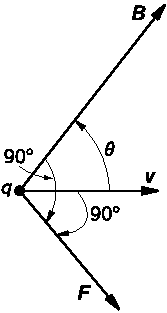
\includegraphics[width=0.3\linewidth]{fyz_fig061.pdf}
      \caption{Složka síly působící na pohybující se náboj závislá na rychlosti je kolmá na 
               \(\vec{v}\) a na směr \(\vec{B}\). Je úměrná složce \(\vec{v}\) kolmé na 
               \(\vec{B}\), tj. úměrná v \(\sin\vartheta\). O existenci magnetické síly se snadno 
                přesvědčíme, přiložíme-li tyčový magnet těsně k obrazovce. Vychýlení elektronového 
                paprsku svědčí o tom, že přítomnost magnetuje projevuje silou působící na 
                elektrony, která je kolmá na směr jejich pohybu, jak to bylo popsáno v kapitole 
                \ref{fyz:IchapXII}, odstavci \ref{fyz:IchapXIIsecIV}.
                \cite[s.~225]{Feynman02}}
      \label{fyz:fig061}
    \end{figure}
    
    Jednotka magnetického pole je zřejmě \(\text{newton}\cdot\text{sekunda}\) na \(\text{coulomb} 
    \cdot \text{metr}\). A stejnou jednotkou je i \(\text{volt}\cdot\text{sekunda}\) na metr 
    čtvereční. Nazývá se \emph{weber na metr čtvereční} nebo \emph{tesla}.

    \subsection{Elektrický proud, zachování náboje}
      \cite[s.~225]{Feynman02} Zamyslíme se nad tím, jak je možné chápat magnetické síly působící 
      na vodiče, jimiž tečou elektrické proudy. Musíme si ujasnit, co budeme chápat pod proudovou 
      hustotou. Elektrické proudy, to jsou elektrony nebo jiné náboje pohybující se takovým 
      způsobem, že v souhrnu vytváří tok v jistém směru. Hustotu toku náboje můžeme charakterizovat 
      vektorem, který určuje množství náboje procházejícího za jednotku času jednotkovou plochou 
      povrchovým elementem kolmým na směr toku (stejně jako v případě tepelného toku). Takovýto tok 
      nazýváme proudová hustota a označujeme jej vektorem \(\vec{j}\) Tento vektor směřuje podél 
      pohybu náboje. Zvolíme-li malou plošku \(\Delta S\) v daném místě látky, množství náboje 
      protékající touto ploškou za jednotku času můžeme vyjádřit ve tvaru
      \begin{equation}\label{eq_fyz:mag001}
        \vec{j}\cdot\vec{n}\Delta S,
      \end{equation} 
      kde \(\vec{n}\) je jednotkový vektor normály k ploše \(\Delta S\).
      
      Proudová hustota souvisí se střední rychlostí toku nábojů. Předpokládejme takové rozdělení 
      nábojů, které vede k usměrněnému pohybu se střední hodnotou rychlosti \(v\). Prochází-li 
      toto rozdělení povrchovým elementem \(\Delta S\), je náboj \(\Delta q\) procházející za čas 
      \(\Delta t\) povrchovým elementem roven náboji obsaženému v rovnoběžnostěnu se základnou 
      \(\Delta S\) a výškou \(v\Delta t\), jak to ukazuje obr. \ref{fyz:fig216}.
      \begin{figure}[ht!]
        \centering
        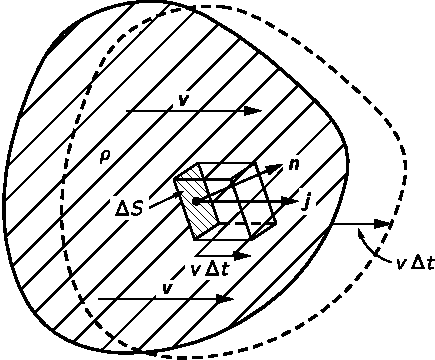
\includegraphics[width=0.7\linewidth]{fyz_fig216.pdf}
        \caption{Pohybuje-li se náboj rozložený s hustotou \(\varrho\) rychlostí \(v\), projde za 
        jednotku času plochou \(\Delta S\) náboj \(\varrho\vec{v}\cdot\vec{n}\Delta S\)}
        \label{fyz:fig216} 
      \end{figure}
      
      Objem tohoto rovnoběžnostěnu je součinem dvou faktorů, z nichž jeden je \(v\Delta t\) druhý 
      je průmět \(\Delta S\) do roviny kolmé na \(\vec{v}\). Násobíme-li tento objem hustotou 
      náboje \(\varrho\), dostaneme \(\Delta q\). Proto můžeme psát
      \begin{equation}\label{eq_fyz:mag002}
        \Delta q = \varrho\vec{v}\cdot\vec{n}\Delta S\Delta t.
      \end{equation}
      Náboj, který prošel za jednotku času, je pak roven \(\varrho\vec{v}\cdot\vec{n}\Delta S\), a 
      proto máme
      \begin{equation}\label{eq_fyz:mag003}
        \vec{j} = \varrho\vec{v}.
      \end{equation}
      
      Skládá-li se rozdělení nábojů z jednotlivých nábojů, např elektronů, z nichž každý má náboj 
      \(q\) a pohybují se střední rychlostí \(v\), můžeme proudovou hustotu vyjádřit ve tvaru
      \begin{equation}\label{fyz:eq808}
        \vec{j} = Nq\vec{v}.
      \end{equation}
      
      Celkový náboj procházející za jednotku času nějakou plochou \(S\) se nazývá \emph{elektrický 
      proud} .Je roven integrálu normálové složky toku všemi elementy povrchu (obr. 
      \ref{fyz:fig217}):
      \begin{equation}\label{fyz:eq807}
        I = \int\vec{j}\cdot\vec{n}\dd{S}.
      \end{equation}
    
      \begin{figure}[ht!]
        \centering
        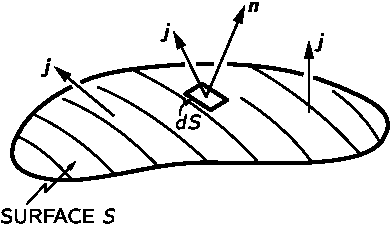
\includegraphics[width=0.5\linewidth]{fyz_fig217.pdf}
        \caption{Proud \(I\) procházející plochou \(S\) je roven \(\int\vec{j}\cdot\vec{n}\dd{S}\)}
        \label{fyz:fig217} 
      \end{figure}
      Proud vycházející z uzavřené plochy \(S\) představuje rychlost, s níž náboj opouští objem 
      \(V\) ohraničený plochou \(S\). Jeden ze základních fyzikálních zákonů hovoří o tom, že 
      elektrický náboj je nezničitelný, nikdy se neztrácí a nevzniká. Elektrické náboje se mohou 
      pohybovat z místa na místo, ale nikdy se neobjevují z ničeho nic. Říkáme, že náboj se 
      zachovává. Vytéká-li v konečném důsledku z uzavřené plochy proud, musí se odpovídajícím 
      způsobem zmenšovat množství náboje v objemu ohraničeném touto plochou (obr. 
      \ref{fyz:fig218}). Zákon zachování náboje proto lze vyjádřit ve tvaru
      \begin{equation}\label{fyz:eq_mag004} 
        \limitoint_{\mathclap{\substack{\text{libovolná}\\\text{uzavřená}\\\text{plocha}}}}
        \vec{j}\cdot\vec{n}\dd{S} = -\der{Q}{t}.
      \end{equation} 
      \begin{figure}[ht!]
        \centering
        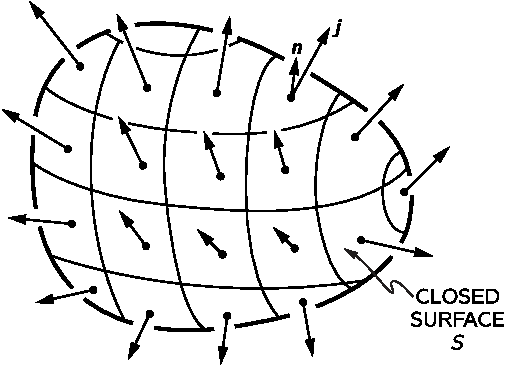
\includegraphics[width=0.5\linewidth]{fyz_fig218.pdf}
        \caption{Integrály \(\vec{j}\cdot\vec{n}\) přes uzavřenou plochu je roven rychlosti změny 
                 celkového náboje \(Q\) uvnitř této plochy.}
        \label{fyz:fig218} 
      \end{figure}
      Vnitřní náboj můžeme vyjádřit jako objemový integrál hustoty náboje
      \begin{equation}\label{fyz:eq_mag005} 
        Q_{\text{uvnitř}} = 
         \limitint_{\mathclap{\substack{V\\\text{uvnitř}\\\text{S}}}}\varrho\dd{V}.
      \end{equation}
      
      Použijeme-li vztah (\ref{fyz:eq_mag004}) pro malý objem \(\dd{V}\), integrál na levé straně 
      (\ref{fyz:eq_mag004}) je roven \(\nabla\cdot\vec{j}\Delta V\). Vnitřní náboj je 
      \(\varrho\Delta V\) a proto zákon zachování náboje lze napsat i ve tvaru
      \begin{equation}\label{fyz:eq_mag006}    %\ref{fyz:eq_mag006}
        \nabla\cdot\vec{j} = -\pder{\varrho}{t}
      \end{equation}
      (Opět \hyperlink{fyz:IIchapIIIsecIII}{Gaussova věta} z matematiky!)

    \subsection{Magnetická síla působící na proud}
      \cite[s.~227]{Feynman02} Nyní už jsme připraveni k tomu, abychom určili sílu, jež působí v 
      magnetickém poli na vodič, kterým teče proud. Proud se skládá z nabitých částic, které se 
      pohybují podél vodiče rychlostí \(v\). Na každý náboj působí příčná síla (obr. 
      \ref{fyz:fig219}).
      \begin{equation}\label{fyz:eq_mag007}
        \vec{F} = q\vec{v}\times\vec{B}
      \end{equation}
      \begin{figure}[ht!]
        \centering
        \subcaptionbox{\label{fyz:fig219a}}{\luafigure[0.45]{fyz_fig219a.pdf}}
        \subcaptionbox{\label{fyz:fig219b}}{\luafigure[0.45]{fyz_fig219b.pdf}}
        \caption{Magnetická síla působící na vodič, jímž protéká proud, je rovna součtu sil 
                 působících na jednotlivé pohybující se náboje}
        \label{fyz:fig219} 
      \end{figure}
      Je-li v objemové jednotce \(N\) takových nábojů, pak v malém objemu vodiče je jich \(N\Delta 
      V\). Celková magnetická síla \(\Delta F\) působící na objem \(\Delta V\) je součtem sil 
      působících na jednotlivé náboje, tj.
      \begin{equation}\label{fyz:eq_mag008}
        \Delta\vec{F} = (N\Delta V)(q\vec{v}\times\vec{B}).
      \end{equation}
      Jenže \(Nqv\) je právě \(\vec{j}\), a proto
      \begin{equation}\label{fyz:eq_mag009}
      \Delta\vec{F} = \vec{j}\times\vec{B}\Delta V.
      \end{equation}
      Jestliže vodičem, jehož plocha příčného řezu je rovna \(S\), teče proud rovnoměrně, můžeme 
      za objemový element zvolit válec se základnou \(S\) a délkou \(\Delta L\). Potom
      \begin{equation}\label{fyz:eq_mag010}
      \Delta\vec{F} = \vec{I}\times\vec{B}\Delta L.
      \end{equation}
      Síla působící na jednotkovou délku vodiče je rovna \(\vec{I}\times\vec{B}\).
      
      Tato rovnice vyjadřuje důležitý výsledek, který spočívá v tom, že magnetická síla působící 
      na vodič proto, že se v něm pohybují náboje, závisí jen na celkovém proudu, a ne na množství 
      náboje neseného každou z částic nebo dokonce na jeho znaménku! Magnetická síla, která v 
      blízkosti magnetu působí na vodič, se projeví vychýlením vodiče při zapnutí proudu tak, jak 
      to bylo popsáno v kapitole \ref{fyz:IIchapI} (obr. \ref{fyz:fig148})

    \subsection{Magnetické pole stacionárních proudů, Ampérův zákon}
      Viděli jsme, že na vodič v magnetickém poli vytvářeném např. magnetem působí síla. Podle 
      zákona akce a reakce bychom mohli očekávat, že bude existovat síla působící na zdroj 
      magnetického pole, tj. na magnet, když vodičem protéká proud\footnote{Později však uvidíme, 
      že takovýto předpoklad není obecně správný pro elektromagnetické síly!}. Takové síly opravdu 
      existují a můžeme se o nich přesvědčit pozorováním odklonu střelky kompasu v blízkosti 
      vodiče, jímž prochází elektrický proud. Dále víme, že mezi magnety existuje silové působení, 
      a proto můžeme usuzovat, že vodič sám vytváří magnetické pole, když jím teče proud. 
      Pohybující se náboje tedy \emph{vytvářejí} magnetické pole. Nyní se pokusme najít zákony, 
      jež určují, jaká pole se vytvoří. Otázka zní: Je-li dán proud, jaké bude magnetické pole jím 
      vytvořené? Odpověď na tuto otázku daly tři kritické experimenty a Ampérův důmyslný 
      teoretický důkaz. Přeskočíme tento zajímavý historický vývoj a pouze se zmíníme o tom, že 
      platnost Maxwellových rovnic byla dokázána velkým počtem experimentů. Maxwellovy rovnice 
      budou naším výchozím bodem. Zanedbáme-li v těchto rovnicích členy obsahující derivace podle 
      času, dostaneme rovnice magnetostatiky.
      \begin{subequations}
        \begin{align}
          \nabla\cdot\vec{B}     &= 0                            \label{fyz:eq_mag011} \\
          c^2\nabla\times\vec{B} &= \frac{\vec{j}}{\epsilon_0}.  \label{fyz:eq_mag012}
        \end{align}
      \end{subequations}
      Tyto rovnice platí jen tehdy, jsou-li všechny hustoty elektrických nábojů konstantní a 
      všechny proudy stacionární, takže elektrická a magnetická pole se s časem nemění - obě pole 
      jsou \emph{stacionární}
      
      Je třeba poznamenat, že předpoklad statické magnetické situace není docela oprávněn, neboť 
      ke vzniku magnetického pole jsou potřebné proudy - a proudy vznikají pouze při pohybu nábojů. 
      Magnetostatika je proto pouze \emph{aproximací}. Souvisí se speciálním druhem dynamické 
      situace, kdy se pohybuje \emph{velký počet} nábojů a tento pohyb lze aproximovat 
      \emph{ustáleným} tokem náboje. Jen tehdy můžeme hovořit o proudové hustotě \(\vec{j}\), 
      která se v čase nemění. Kdybychom chtěli být přesnější, měli bychom tuto část nazývat 
      zkoumáním stacionárních proudů. Předpokládáme-li stacionárnost všech polí, můžeme v úplném 
      systému Maxwellových rovnic (\ref{fyz:eq266}) vynechat členy s \(\pder{\vec{E}}{t}\) a 
      \(\pder{\vec{B}}{t}\), a tak dostaneme již uvedenou dvojici rovnic (\ref{fyz:eq_mag011}) a 
      (\ref{fyz:eq_mag012}). Všimněte si, že divergence rotace libovolného vektoru je nevyhnutelně 
      nula, a proto rovnice (\ref{fyz:eq_mag012}) vyžaduje, aby \(\nabla\cdot\vec{j} = 0\). 
      Platí-li rovnice (\ref{fyz:eq_mag006}), bude to splněno pouze tehdy, když 
      \(\pder{\varrho}{t}\) rovno nule. To platí tehdy, když se \(\vec{E}\) s časem  nemění, takže 
      naše předpoklady jsou konzistentní.
      
      Podmínka \(\nabla\cdot\vec{j} = 0\) znamená, že můžeme uvažovat jen takové náboje, které se 
      pohybují po \emph{uzavřených dráhách}. Můžou např. téct ve vodičích tvořících uzavřené 
      smyčky, které nazýváme obvody. Obvody mohou, samozřejmě obsahovat generátory nebo baterie, 
      které udržují tok nábojů. Nesmí však obsahovat kondenzátory, které se nabíjejí nebo 
      vybíjejí. (Později, samozřejmě, rozšíříme teorii i na dynamická pole, ale nejdříve se budeme 
      zabývat jednodušším případem stacionárních proudů.)
      
      Nyní si všimneme rovnic (\ref{fyz:eq_mag011}) a (\ref{fyz:eq_mag012}) a zamyslíme se nad 
      tím, co znamenají. První rovnice říká, že divergence \(\vec{B}\) je rovna nule. Porovnáme-li 
      ji s analogickou rovnicí elektrostatiky, která říká, že \(\nabla\cdot\vec{E} = 
      \frac{\varrho}{\epsilon_0}\), zjistíme, že neexistuje magnetická analogie elektrického 
      náboje. \textbf{Neexistují magnetické náboje}, z nichž by mohly vycházet čáry \(\vec{B}\). 
      Budeme-li v našich úvahách používat pojem \emph{„indukční čáry“} vektorového pole 
      \(\vec{B}\), tyto nebudou nikde začínat a nikde končit. Odkud tedy pocházejí? Magnetická 
      pole se \emph{„objevují“} v \emph{přítomnosti} proudů; mají rotaci úměrnou proudové hustotě. 
      Kdekoliv jsou proudy, jsou tam i čáry magnetického pole vytvářející smyčky okolo proudů. 
      Protože čáry \(\vec{B}\) nezačínají a nekončí, často se uzavírají do sebe a vytvářejí 
      uzavřené smyčky. Mohou však existovat složité situace, v nichž čáry nejsou jednoduchými 
      uzavřenými smyčkami. Ale ať procházejí kudykoliv, nikdy nevycházejí z bodů. Magnetické 
      náboje nebyly nikdy objeveny, a proto \(\nabla\cdot\vec{B} = 0\). Platí to vždy - nejen pro 
      \emph{magnetostatiku}, ale i pro \emph{dynamická pole}.
      
      Souvislost mezi polem \(\vec{B}\) a proudy je vyjádřen rovnicí (\ref{fyz:eq_mag012}). Máme 
      novou situaci, zcela odlišnou od elektrostatiky, kde platilo \(\nabla\times\vec{E}=0\). 
      Takový vztah znamenal, že křivkový integrál z \(\vec{E}\) po libovolné uzavřené dráze je 
      roven nule:
      \begin{equation}\label{fyz:eq_mag013} 
        \limitoint_{\mathclap{\substack{\text{po smyčce}}}}\vec{E}\cdot\dd{\vec{s}} = 0.
      \end{equation} 
      Tento výsledek jsme získali ze \hyperlink{fyz:IIchapIIIsecV}{Stokesovy věty}, která říká, že 
      integrál po libovolné uzavřené dráze jakéhokoliv vektorového pole je roven plošnému 
      integrálu normálové složky rotace vektoru (integrál bereme po libovolné ploše, která má jako 
      svou hranici uzavřenou smyčku). Kdybychom tutéž větu použili v případě vektoru magnetického 
      pole, dostali bychom použitím symbolů z obr. \ref{fyz:fig220}.
      \begin{equation}\label{fyz:eq_mag014} 
        \limitoint_{\mathclap{\substack{\Gamma}}}\vec{B}\dd{\vec{s}} = 
        \limitint_{\mathclap{\substack{S}}}(\nabla\times\vec{B})\cdot\vec{n}\dd{S}.
      \end{equation}       
      Vezmeme-li rotaci \(\vec{B}\) rovnice (\ref{fyz:eq_mag012}), dostaneme
      \begin{equation}\label{fyz:eq801}
        \limitoint_{\mathclap{\substack{\Gamma}}}\vec{B}\dd{\vec{s}} = 
        \dfrac{1}{ϵ_0c^2}\limitint_{\mathclap{\substack{S}}}\vec{j}\cdot\vec{n}\dd{S}.
      \end{equation}
      \begin{figure}[ht!]
        \centering
        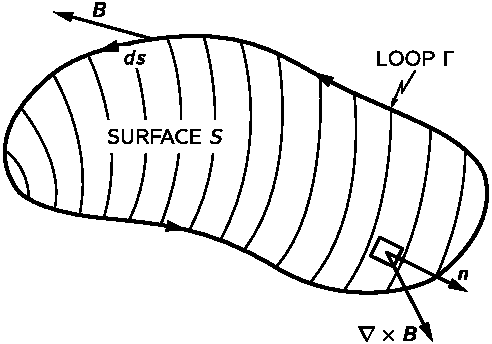
\includegraphics[width=0.7\linewidth]{fyz_fig220.pdf}
        \caption{Křivkový integrál tangenciální složky \(\vec{B}\) je roven plošnému integrálu 
                 normálové složky \(\nabla\times\vec{B}\).}
        \label{fyz:fig220} 
      \end{figure}
      Souhlasně se vztahem (\ref{fyz:eq807}) představuje integrál \(j\) celkový proud \(I\)
      tekoucí plochou \(S\). Protože v případě stacionárních proudů nezávisí proud plochou \(S\) na
      tvaru této plochy, pokud je ohraničena křivkou \(\Gamma\), hovoříme o \emph{proudu smyčkou}
      \(\Gamma\). Tak přicházíme k obecnému zákonu: Cirkulace \(\vec{B}\) podél libovolné uzavřené
      křivky je rovna proudu \(I\) smyčkou \(\Gamma\) dělenému \(ϵ_0c^2\)
      \begin{equation}\label{fyz:eq802}
        \limitoint_{\mathclap{\substack{\Gamma}}}\vec{B}\dd{\vec{s}} = 
        \dfrac{I_{\text{smyčkou }\Gamma}}{ϵ_0c^2}.
      \end{equation}
      Tento zákon - zvaný \textbf{Ampérův zákon} - hraje v magnetostatice tutéž úlohu jako Gaussův
      zákon v elektrostatice. Samotný Ampérův zákon neurčuje \(\vec{B}\) z proudů; obecně musíme
      použít i vztah \(\nabla\times\vec{B} = 0\). V další části však uvidíme, že jej můžeme použít i
      pro určení polí v takových speciálních případech, které mají určitou jednoduchou symetrii.

  \section{Magnetické pole přímého vodiče a solenoidu. Atomové proudy}\label{fyz:IIchapXIIIsecV}
    Abychom ukázali, jak lze Ampérův zákon použít, určíme magnetické pole v blízkosti vodiče. Ptáme
    se: Jaké je pole v okolí dlouhého přímého vodiče válcového tvaru? Budeme předpokládat něco, co
    vůbec nemusí být zřejmé, ale přece je to pravdivé: že indukční čáry pole \(\vec{B}\) vytvářejí
    okolo vodiče kružnice. Za takového předpokladu Ampérův zákon, tj. rovnice (\ref{fyz:eq802}),
    určuje sílu pole. V důsledku symetrie úlohy má \(\vec{B}\) stejnou velikost ve všech bodech
    kružnice, jejíž střed je v ose vodiče (obr. \ref{fyz:fig683}). Pak můžeme snadno vypočítat
    integrál \(\vec{B}\cdot\dd{s}\); je roven právě velikosti \(\vec{B}\) násobené délkou kružnice.
    Je-li \(r\) poloměr kružnice, máme
    \begin{equation}\label{fyz:eq803}
      \limitoint_{\mathclap{\substack{\Gamma}}}\vec{B}\dd{\vec{s}} = B\cdot2\pi r.
    \end{equation}

    \begin{figure}[ht!] %\ref{fyz:fig683}
      \centering
      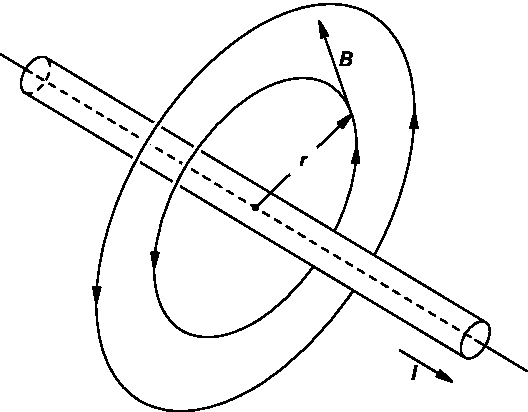
\includegraphics[width=0.7\linewidth]{fyz_fig683.pdf}
      \caption{Magnetické pole v okolí dlouhého vodiče, jímž prochází proud \(I\)
              (\cite[s.~707]{Feynman02})}
      \label{fyz:fig683}
    \end{figure}

    Celkový proud smyčkou je prostě proud \(I\) ve vodiči, a proto
    \begin{equation*}
      B\cdot2\pi r = \dfrac{I}{\varepsilon_0c^2}.
    \end{equation*}
    nebo
    \begin{equation}\label{fyz:eq804}
      B = \dfrac{1}{4\pi\varepsilon_0c^2}\dfrac{2I}{r}.
    \end{equation}  
    Velikost magnetického pole klesá nepřímo úměrně \(r\) - vzdálenosti od osy vodiče. Chceme-li,
    můžeme vztah (\ref{fyz:eq804}) zapsat ve vektorovém tvaru. Uvědomíme si, že \(\vec{B}\) je kolmé
    jak na \(\vec{I}\), tak na \(\vec{r}\) a dostaneme
    \begin{equation}\label{fyz:eq805}
      \vec{B} = \dfrac{1}{4\pi\varepsilon_0c^2}\dfrac{2\vec{I}\times\vec{e}_r}{\vec{r}}.
    \end{equation} 
    Faktor \(\dfrac{1}{4\pi\varepsilon_0c^2}\) píšeme odděleně proto, že se bude vyskytovat často.
    Bude dobré, když si zapamatujete, že je roven přesně \num{e-7} (v SI soustavě), neboť rovnicí
    typu (\ref{fyz:eq805}) je \emph{definována} jednotka proudu - \textbf{ampér}. Ve vzdálenosti
    jednoho metru od vodiče s proudem jednoho ampéru je magnetické pole \num{2e-7} tesla.

    \begin{figure}[ht!] %\ref{fyz:fig684}
      \centering
      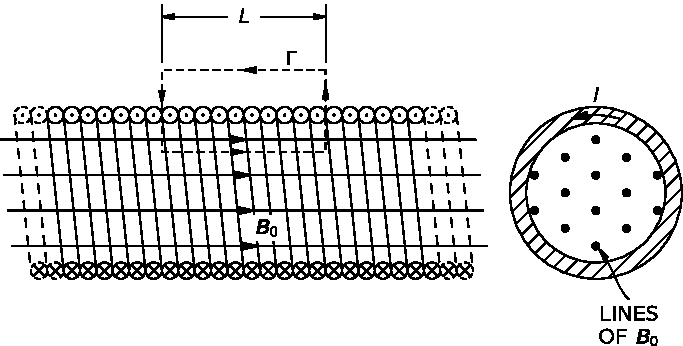
\includegraphics[width=1\linewidth]{fyz_fig684.pdf}
      \caption{Magnetické pole dlouhého solenoidu
               (\cite[s.~707]{Feynman02})}
      \label{fyz:fig684}
    \end{figure}

    Protože proud vytváří magnetické pole, bude působitsilou na okolní vodiče, jimiž také protéká
    proud. V kapitole \ref{fyz:IIchapI} byl popsán jednoduchý pokus na demonstraci síly působící
    mezi dvěma vodiči proudu. Jsou-li vodiče rovnoběžné, je každý kolmý na pole druhého vodiče;
    vodiče se proto budou odpuzovat, nebo přitahovat. Tečou-li proudy stejným směrem, vodiče se
    přitahují; mají-li proudy směr opačný, vodiče se odpuzují.

    Všimněme si jiného příkladu, při jehož analýze nám pomůže Ampérův zákon a určité poznatky o
    povaze pole. Předpokládejme, že máme dlouhý drát v podobě cívky těsně navinutý na válcové ploše
    tak, jak je znázorněno v řezu na obr. \ref{fyz:fig684}. Taková cívka se nazývá solenoid. Je-li
    solenoid vzhledem ke svému průměru velmi dlouhý, lze experimentálně zjistit, že pole v okolí
    solenoidu je velmi malé v porovnání s polem uvnitř solenoidu. Použitím této skutečnosti a
    Ampérova zákona můžeme určit velikost pole uvnitř solenoidu.

    Protože pole zůstává uvnitř (a má nulovou divergenci), musí jeho indukční čáry jít rovnoběžně s
    osou, jak znázorňuje obr. \ref{fyz:fig685}. Je-li to tak, můžeme použít Ampérův zákon na
    pravoúhlou křivku \(\Gamma\) znázorněnou na obrázku.

    \begin{figure}[ht!] %\ref{fyz:fig685}
      \centering
      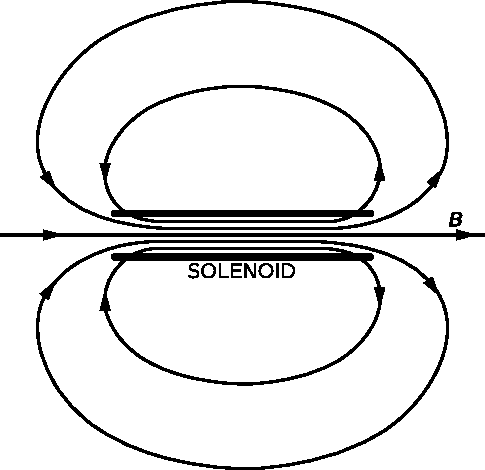
\includegraphics[width=0.7\linewidth]{fyz_fig685.pdf}
      \caption{Magnetické pole v okolí solenoidu
               (\cite[s.~707]{Feynman02})}
      \label{fyz:fig685}
    \end{figure}

    Tato smyčka prochází vzdálenost \(L\) uvnitř solenoidu, kde je pole řekněme \(\vec{B}_0\) potom
    jde kolmo k poli a vrací se podél solenoidu vnější stranou, kde je pole zanedbatelné. Křivkový
    integrál \(\vec{B}\) podél této křivky je roven právě \(B_0L\), což musí být rovno celkovému
    proudu, který obepíná křivka \(\Gamma\) vynásobenému faktorem \(l/\varepsilon_0c^2\). Má-li
    solenoid \(N\) závitů na délce \(L\), bude obepínaný proud \(NI\). Máme tedy
    \begin{equation*}
      B_0L = \dfrac{NI}{\varepsilon_0c^2}.
    \end{equation*}
    Označíme-li symbolem \(n\) počet závitů solenoidu na jednotkové délce (tj. \(n = N/L\)),
    dostaneme
    \begin{equation}\label{fyz:eq806}
      B_0 = \dfrac{nI}{\varepsilon_0c^2}.
    \end{equation}

    Co se stane s indukčními čarami \(\vec{B}\), když se dostanou na konec solenoidu? Zřejmě se
    nějak rozejdou a vrátí se k solenoidu na opačném konci tak, jak je to nakresleno na obr.
    \ref{fyz:fig685}.

    Ale právě takové pole pozorujeme i v okolí tyčového magnetu. Co je však vlastně magnet? Naše
    rovnice říkají, že \(\vec{B}\) je důsledkem přítomnosti proudů. Víme i to, že obyčejné železné
    tyče (bez baterií a generátorů) také vytvářejí magnetická pole. Možná očekáváme, že na pravé
    straně rovnic (\ref{fyz:eq_mag011}) a (\ref{fyz:eq_mag011}) by měly být ještě další členy, které
    by představovaly „hustotu magnetického železa“ nebo nějakou jinou podobnou veličinu. Takové
    členy tam nejsou. Naše teorie říká, že za magnetické vlastnosti železa jsou odpovědné vnitřní
    proudy, které jsou už zahrnuty ve členu s \(\vec{j}\).

    Látky jsou velmi složité, zkoumáme-li hlouběji; to jsme viděli, když jsme se snažili pochopit 
    dielektrika. Abychom nepřerušili tuto naši diskusi, odložíme podrobné zkoumání vnitřního
    mechanizmu magnetických materiálů typu železa na později. Zatím se budete muset smířit s tím, že
    všechen magnetizmus je tvořen proudy a že v permanentním magnetu jsou stálé vnitřní proudy. V
    případě železa tyto proudy pocházejí od elektronů rotujících okolo vlastních os. Každý elektron
    má spin, který odpovídá maličkému cirkulujícímu proudu. Samozřejmě, jeden elektron nevytvoří
    znatelné magnetické pole, ale v obyčejném kusu látky jsou miliardy a miliardy elektronů. Obvykle
    elektrony rotují v těch nejrozmanitějších směrech, a proto se výsledný efekt neprojevuje.
    Kupodivu v malém počtu látek podobných železu rotuje velká část elektronů tak, že jejich osy
    rotace mají stejný směr - v železe se takového kolektivního pohybu účastní dva elektrony každého
    atomu. V tyčovém magnetu rotuje velký počet elektronů ve stejném směru a jak uvidíme později,
    výsledný jev je rovnocenný proudu cirkulujícímu na povrchu magnetu. (Je to velmi podobné tomu,
    co jsme zjistili v dielektrikách - že rovnoměrně polarizované dielektrikum je ekvivalentní
    rozložení nábojů na jeho povrchu.) Není tedy náhoda, že tyčový magnet je ekvivalentní se
    solenoidem.

  \section{Magnetická a elektrická pole v teorii relativity}\label{fyz:IIchapXIIIsecVI}
    Když jsme říkali, že magnetická síla působící na náboj je úměrná jeho rychlosti, možná, že jsme
    si položili otázku: \uv{Jaké rychlosti? Vzhledem, ke které vztažné soustavě?} Z definice
    veličiny \(\vec{B}\), uvedené na začátku této kapitoly, skutečně vyplývá, že tento vektor bude
    záviset na volbě vztažné soustavy při určování rychlosti nábojů. O tom, kterou soustavu je třeba
    při určování magnetického pole brát v úvahu, jsme však neřekli nic.
    
    \begin{figure}[ht!]  %\ref{fyz:fig686}
      \centering
      \subcaptionbox{\label{fyz:fig686a}}{\luafigure[1]{fyz_fig686a.pdf}} \\
      \subcaptionbox{\label{fyz:fig686b}}{\luafigure[1]{fyz_fig686b.pdf}}
      \caption{Interakce vodiče, kterým teče proud, a částice s nábojem \(q\) z hlediska dvou
              souřadnicových soustav. V soustavě \(S\) (část a) je vodič v klidu; v soustavě \(S'\)
              (část b) je v klidu náboj. (\cite[s.~234]{Feynman02})}
      \label{fyz:fig686}
    \end{figure}

    Ukazuje se, že je vhodná \emph{libovolná} inerciální soustava. Také uvidíme, že magnetizmus a
    elektřina nejsou navzájem nezávislé - je třeba je chápat jako součást jednoho úplného
    elektromagnetického pole. Ačkoliv se ve statickém případě Maxwellovy rovnice rozpadnou na dva
    samostatné páry, jeden pro elektřinu a druhý pro magnetizmus, a mezi těmito dvěma poli pak není
    zjevná souvislost, přece v samotné přírodě mezi nimi existuje velmi úzký vztah, který je
    důsledkem principu relativity. Historicky byl princip relativity objeven později než Maxwellovy
    rovnice. Bylo to vlastně studium elektřiny a magnetizmu, které nakonec Einsteina přivedlo k
    objevu principu relativity. Všimněme si, co nám naše poznání principu relativity řekne o
    magnetických silách, předpokládáme-li, a to zcela správně, že princip relativity lze při
    zkoumání elektromagnetizmu použít.

    Zamysleme se nad tím, co se stane, bude-li se záporný náboj pohybovat rychlostí \(v_0\)
    rovnoběžně s vodičem, kterým teče proud (situace je znázorněna na obr. \ref{fyz:fig686}). Budeme
    se snažit pochopit situaci ve dvou vztažných soustavách: jedné spojené s vodičem tak jako na
    obr. \ref{fyz:fig686a} a druhé spojené s částicí tak jako na obr. \ref{fyz:fig686b}. První
    soustavu označíme symbolem \(S\) a druhou symbolem \(S'\).

    V soustavě \(S\) na částici zřejmě působí magnetická síla. Síla směřuje k vodiči, takže kdyby se
    náboj volně pohyboval, viděli bychom ho stáčet se k vodiči. V soustavě \(S'\) však na částici
    magnetická síla nepůsobí, neboť částice má nulovou rychlost. Zůstane proto stát na místě?
    Uvidíme v těch dvou soustavách různé události? Podle principu relativity bychom měli i v
    soustavě \(S'\) vidět částici přibližující se k vodiči. Musíme vysvětlit, proč by to tak mělo
    být.

    Vraťme se k našemu atomovému popisu vodiče, který vede proud. V normálním vodiči, jakým je měď,
    vzniká elektrický proud pohybem určitého počtu záporných elektronů (nazýváme je vodivostní
    elektrony), zatímco kladné náboje jader a zbytek elektronů jsou v materiálu nepohyblivé. Označme
    hustotu vodivostních elektronů \( ρ_−\) a jejich rychlost v soustavě \(S\) jako \(v\). Hustota
    nábojů, které se v \(S\) nepohybují, nechť je \( ρ_+\) a ta musí být rovna \( ρ_−\) s opačným
    znaménkem, neboť  máme nenabitý vodič. Proto mimo vodič nebude existovat elektrické pole a síla
    působící na pohybující se částici je rovna
    \begin{equation*}
      \vec{F}=q\vec{v}_0\times\vec{B}.
    \end{equation*}
    Využijeme-li výsledek, ke kterému jsme přišli v rovnici (\ref{fyz:eq804}) pro magnetické pole ve
    vzdálenosti \(r\) od osy vodiče, dospějeme k závěru, že síla působící na částici směřuje k
    vodiči a má velikost
    \begin{equation*}
      F=\dfrac{1}{4πϵ_0c^2}\cdot\dfrac{2Iqv_0}{r}.
    \end{equation*}
    Pomocí rovnic (\ref{fyz:eq807}) a (\ref{fyz:eq808}) můžeme proud /vyjádřit ve tvaru
    \(ρ_−vS\), kde \(S\) je plošný obsah průřezu vodiče. Potom
    \begin{equation}\label{fyz:eq809}
      F=\dfrac{1}{4πϵ_0c^2}\cdot\dfrac{2qρ_−Svv_0}{r}.
    \end{equation}

    Mohli bychom pokračovat ve zkoumání obecného případu libovolných rychlostí \(v\) a \(v_0\), ale
    stejně dobře bude, všimneme-li si speciálního případu, kdy rychlost částice \(v_0\) je stejná
    jako rychlost vodivostních elektronů \(v\). Potom můžeme psát \(v=v_0\) a rovnice
    (\ref{fyz:eq809}) se změní na
    \begin{equation}\label{fyz:eq810}
      F=\dfrac{q}{2πϵ_0}\cdot\dfrac{ρ_−S}{r}\dfrac{v^2}{c^2}.
    \end{equation}

    Zajímáme se o to, co se stane v soustavě \(S'\), v níž je částice v klidu a pohybuje se vodič
    (na  obrázku \ref{fyz:fig686b} doleva) rychlostí \(v\). Kladné náboje pohybující se s vodičem
    vytvoří určité magnetické pole  \(B'\) v okolí částice. Jenže částice je nyní v klidu, a proto
    na ni nepůsobí \emph{magnetická} síla! Působí-li na částici přece jen nějaká síla, musí pocházet
    od elektrického pole. To je však možné pouze tehdy, když je vodič \emph{nabitý} - neutrální
    vodič, kterým protéká proud se musí stát nabitým, když jej uvedeme do pohybu.

    Tuto otázku musíme prozkoumat. Pomocí toho, co víme o soustavě \(S\), musíme určit hustotu
    náboje ve vodiči v soustavě \(S'\). Na první pohled vypadá všechno stejně, ale už víme, že při
    přechodu z \(S\) do \(S'\) se mění délky (\ref{fyz:IchapXV}. kapitola \ref{part:FYZI}. dílu);
    proto se musí měnit i objemy. Musí se tedy změnit i hustoty, neboť \emph{hustoty} náboje
    závisejí na objemu, v němž se náboje nacházejí.

    Dřív než určíme hustoty náboje v \(S'\), musíme vědět, co se děje s elektrickým \emph{nábojem}
    svazku elektronů, když se náboje pohybují. Víme, že hmotnost částice roste v poměru \(1/\sqrt{1
    - v^2/c^2}\).  Děje se něco podobného i s nábojem? Ne! Náboje jsou vždy stejné bez ohledu na to,
    zda se pohybují nebo nepohybují. Jinak bychom nepozorovali, že se celkový náboj zachovává.

    Předpokládejme, že máme kousek materiálu, řekněme vodiče, který byl původně nenabitý. 
    Zahřejeme ho. Protože elektrony mají jiné hmotnosti než protony, změní se rychlosti elektronů a
    protonů různě. Závisel-li by náboj na rychlosti částice, která ho nese, nebyl by už v ohřátém
    kousku materiálu náboj elektronů a protonů v rovnováze. Při zahřátí by se materiál nabil. Jak
    jsme už viděli dříve, velmi malá změna náboje každého z elektronů by vedla v takovém kousku
    materiálu k obrovským elektrickým polím. Takový jev však nebyl nikdy pozorován.

    Je tu ještě ta skutečnost, že střední rychlost elektronů v látce závisí na jejím chemickém
    složení. Kdyby se náboj elektronu měnil s rychlostí, výsledný náboj látky by se měnil v chemické
    reakci. Přímý výpočet by nám opět ukázal, že i velmi malá závislost náboje na rychlosti by vedla
    v nejjednodušších chemických reakcích k obrovským elektrickým polím. Takové jevy však nebyly
    pozorovány, a proto můžeme tvrdit, že elektrický náboj jednotlivých částic nezávisí na jejich
    pohybovém stavu.

    Náboj částice \(q\) je tedy invariantní skalární veličina, nezávislá na vztažné soustavě. To
    znamená, že v libovolné soustavě je hustota náboje nějakého rozdělení elektronů úměrná počtu
    elektronů v jednotce objemu. Starosti nám bude dělat jen skutečnost, že objem se múze měnit v
    důsledku relativistické kontrakce délek.

    Tuto myšlenku použijeme v případě pohybujícího se vodiče. Vezmeme-li vodič délky \(L_0\) v němž
    je hustota \emph{stacionárních} nábojů \(\varrho_0\), bude obsahovat celkový náboj
    \(Q=ρ_0L_0S_0\). Pohybují-li se tytéž náboje v druhé soustavě rychlostí \(v\) budou se všechny
    nacházet v kousku látky, který má kratší délku:
    \begin{equation}\label{fyz:eq811}
      L=L_0\sqrt{1−v^2/c^2}.
    \end{equation}
    ale tentýž průřez \(S_0\) (protože rozměry v směrech kolmých na pohyb se nemění). Tato situace je
    znázorněna na obr. \ref{fyz:fig687}.

    \begin{figure}[ht!]  %\ref{fyz:fig686}
      \centering
      \subcaptionbox{\label{fyz:fig687a}}{\luafigure[1]{fyz_fig687a.pdf}} \\
      \subcaptionbox{\label{fyz:fig687b}}{\luafigure[1]{fyz_fig687b.pdf}}
      \caption{Má-li rozdělení nabitých částic v klidu hustotu \(\varrho_0\), budou mít tytéž náboje
              hustotu \(ρ=ρ_0\sqrt{1−v^2/c^2}\), budeme-li je pozorovat v soustavě pohybující se
              rychlostí \(v\) vůči nabitým částicím (\cite[s.~236]{Feynman02})}
      \label{fyz:fig687}
    \end{figure}

    Označíme-li symbolem \(\varrho\) hustotu náboje v soustavě, v níž se náboje pohybují, bude
    celkový náboj \(Q\) roven \(ρLS_0\). To však musí být rovno \(ρL_0S_0\), neboť náboj je v každé
    soustavě stejný. Proto \(ρL=ρ_0L_0\), nebo podle \ref{fyz:eq811})
    \begin{equation}\label{fyz:eq812}
      ρ=\dfrac{ρ_0}{\sqrt{1−v^2/c^2}}.
    \end{equation}
    \emph{Hustota} náboje pohybujícího se souboru nábojů se mění stejným způsobem jako
    relativistická hmotnost částice.

    Nyní tento obecný výsledek použijeme na hustotu kladného náboje \(varrho?+\) našeho vodiče. Tyto
    náboje jsou v klidu v soustavě \(S\). V soustavě v níž se vodič pohybuje rychlostí \(v\), bude
    pro hustotu kladného náboje platit vztah
    \begin{equation}\label{fyz:eq813}
      ρ_+'=\dfrac{ρ_+}{\sqrt{1−v^2/c^2}}.
    \end{equation}

    \emph{Záporné náboje} jsou v klidu v soustavě \(S'\). Jejich \uv{klidová hustota} bude v této
    soustavě rovna \(\varrho_0\). V rovnici (\ref{fyz:eq812}) \(\varrho_0 = \varrho_-'\), neboť
    jejich hustota je rovna \(ρ_−\) když je vodič v klidu, tj. v soustavě \(S\), kde je rychlost
    záporných nábojů \(v\). Pro vodivostní elektrony potom máme
    \begin{align}
      ρ_-  &=\dfrac{ρ_-'}{\sqrt{1−v^2/c^2}}. \label{fyz:eq814} \\
      \shortintertext{nebo}
      ρ_-' &=ρ_-\sqrt{1−v^2/c^2}.            \label{fyz:eq815}
    \end{align}

    Teď už je vidět, proč je v soustavě \(S'\) elektrické pole - neboť v této soustavě je výsledná
    hustota náboje \(\varrho'\) ve vodiči dána vztahem
    \begin{equation*}
      ρ′=ρ′_++ρ′_−.
    \end{equation*}
    Použijeme-li (\ref{fyz:eq813}) a (\ref{fyz:eq815}), dostaneme
    \begin{equation*}
      ρ′=\dfrac{ρ_+}{\sqrt{1−v^2/c^2}}+ ρ_−\sqrt{1−v^2/c^2}.
    \end{equation*}
    Protože stacionární vodič je neutrální, platí \(ρ_−=−ρ_+\) a máme
    \begin{equation}\label{fyz:eq816}
      ρ′=ρ_+\cdot\dfrac{v^2/c^2}{\sqrt{1−v^2/c^2}}.
    \end{equation}
    Náš pohybující se vodič je kladně nabitý a vytvoří elektrické pole \(E'\) v bodě, kde se nachází
    vnější stacionární částice. Už jsme vyřešili elektrostatický problém homogenně nabitého válce.
    Elektrické pole ve vzdálenosti \(r\) od osy válce je
    \begin{equation}\label{fyz:eq817}
      E′=\dfrac{ρ′S}{2πϵ_0r} = \dfrac{ρ_+Sv^2/c^2}{2πϵ_0r\sqrt{1−v^2/c^2}}.
    \end{equation}
    Síla působící na záporně nabitou částici směřuje k vodiči. Máme tedy sílu, která alespoň pokud
    jde o směr, je stejná v obou soustavách; elektrická síla v \(S'\) má tentýž směr jako magnetická
    síla v \(S\). Velikost síly v \(S'\) je 
    \begin{equation}\label{fyz:eq818}
      F′=\dfrac{q}{2πϵ_0} = \dfrac{ρ_+S}{r}\dfrac{v^2/c^2}{\sqrt{1−v^2/c^2}}.
    \end{equation}
    Porovnáním výsledku pro \(F'\) s naším výsledkem pro \(F\) z rovnice (\ref{fyz:eq810}) zjistíme,
    že velikosti těchto sil jsou téměř stejné. Skutečně,
    \begin{equation}\label{fyz:eq819}
      F′=\dfrac{F}{\sqrt{1−v^2/c^2}},
    \end{equation}
    a proto při malých rychlostech, které jsme uvažovali, jsou si tyto síly rovny. Lze tedy říci, že
    alespoň při malých rychlostech můžeme magnetizmus a elektřinu považovat za „dva pohledy na tutéž
    věc“.

    Situace je však ještě příznivější. Vezmeme-li v úvahu skutečnost, že i síly se transformují při
    přechodu z jedné soustavy do druhé, zjistíme, že oba způsoby pozorování událostí opravdu dávají
    tentýž \emph{fyzikální} výsledek při libovolné rychlosti.

    Abychom se o tom přesvědčili, položme si otázku: Jakou příčnou hybnost bude mít částice, na
    kterou po krátkou dobu působila síla? Z \ref{fyz:IchapXVI}. kapitoly \ref{part:FYZI}. dílu už
    víme, že příčná hybnost částice musí být stejná v soustavě \(S\) i \(S'\). Označíme-li příčnou
    souřadnici \(y\) budeme porovnávat \(Δp_y\) a \(Δp'_y\). Použijeme-li relativisticky správnou
    pohybovou rovnici \(\vec{F}=\diff{\vec{p}}{t}\), pro příčnou hybnost \(Δp_y\), kterou částice
    získá za dobu \(Δt\) v soustavě \(S\), dostaneme
    \begin{align}
      Δp_y &=FΔt.     \label{fyz:eq820} \\
      \shortintertext{V soustavě \(S'\) bude pro příčnou hybnost platit}
      Δp'_y &=F'Δt'.  \label{fyz:eq821}
    \end{align}
    Veličiny \(Δp_y\) a \(Δp'_y\) musíme samozřejmě porovnávat v odpovídajících časových intervalech
    \(Δt\) a \(Δt'\). V \ref{fyz:IchapXV}. kapitole \ref{part:FYZI}. dílu jsme viděli, že časové
    intervaly vztahující se k \emph{pohybující} se částici jsou \emph{delší} než intervaly v
    soustavě, v níž je částice v klidu. Protože naše částice byla původně v klidu v soustavě \(S'\),
    můžeme pro malé \(Δt\) psát
    \begin{equation}\label{fyz:eq822}
      Δt=\dfrac{Δt'}{\sqrt{1−v^2/c^2}},
    \end{equation}
    a vše krásné vychází. Z rovnic (\ref{fyz:eq820}) a (\ref{fyz:eq821}) dostaneme
    \begin{equation*}
      \dfrac{Δp′_y}{Δpy}=\dfrac{F′Δt′}{FΔt},
    \end{equation*}
    a zkombinováním vztahů (\ref{fyz:eq819}) a (\ref{fyz:eq822}) se můžeme přesvědčit, že tento
    poměr je roven jedné.

    \begin{figure}[ht!] %\ref{fyz:fig688}
      \centering
      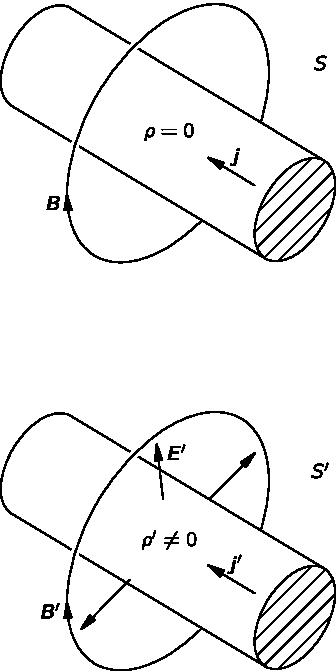
\includegraphics[width=0.7\linewidth]{fyz_fig688.pdf}
      \caption{V soustavě \(S\) je hustota náboje nulová a proudová hustota je rovna \(\vec{j}\). Je
            tam jen magnetické pole. V \(S'\) je hustota náboje \(\varrho_-\) a jiná proudová
            hustota \(\vec{j}'\). Magnetické pole \(\vec{B}'\) je jiné a je tam i elektrické pole
            \(\vec{E}'\). (\cite[s.~238]{Feynman02})}
      \label{fyz:fig688}
    \end{figure}

    Zjistili jsme, že stejný fyzikální výsledek dostaneme při analýze pohybu částice ve vodiči v
    souřadnicové soustavě spojené s vodičem nebo v soustavě spojené s částicí. V prvním případě je
    tato síla čistě „magnetická“ a v druhém čistě „elektrická“. Tyto dva pohledy znázorňuje obr.
    \ref{fyz:fig688}. (I když v druhé soustavě je magnetické pole \(B'\), nepůsobí na stacionární
    částici silou).

    Kdybychom zvolili další souřadnicovou soustavu, dostali bychom jiná pole \(\vec{E}\) a
    \(\vec{B}\). Elektrické a magnetické síly jsou částí \emph{jednoho} fyzikálního jevu -
    elektromagnetické interakce částic. Rozdělení této interakce na elektrickou a magnetickou část
    závisí na tom, jakou vztažnou soustavu jsme zvolili pro popis situace. Teprve úplný
    elektromagnetický popis je invariantní; elektřina a magnetizmus chápané jako celek jsou
    konzistentní s Einsteinovou teorií relativity.

    Protože při změně vztažné soustavy se mění i zastoupení elektrického a magnetického pole, musíme
    být v našich úvahách o polích \(\vec{E}\) a \(\vec{B}\) opatrní. Hovoříme-li například o
    \emph{čarách} \(\vec{E}\) a \(\vec{B}\), nesmíme jim připisovat příliš mnoho reality. Tyto čáry
    se mohou ztratit, chceme-li je pozorovat v jiné souřadnicové soustavě. Například v soustavě
    \(S'\) máme siločáry elektrického pole, ale nenajdeme je, \uv{pohybujeme-li se rychlostí \(v\) v
    soustavě \(S\)}. V soustavě \(S\) nejsou vůbec siločáry elektrického pole! Nemá proto smysl
    vyslovit takovéto nebo podobné tvrzení: Pohybujeme-li magnetem, unáší s sebou své pole, a proto
    se pohybují indukční čáry \(\vec{B}\). Obecně nemá smysl hovořit o \uv{rychlosti pohybujících se
    čar pole}. Pole jsou naším způsobem popisu toho, co se děje v daném bodě prostoru. Konkrétně
    \(\vec{E}\) a \(\vec{B}\) vypovídají o silách, které působí na pohybující se částice. Otázka
    \uv{Jaká je síla působící na náboj ze strany \emph{pohybujícího} se magnetického pole?} nemá
    žádný přesný smysl.  Síla je určována hodnotami \(\vec{E}\) a \(\vec{B}\) v místě náboje a vztah
    (\ref{fyz:eq823}) není třeba měnit, pohybuje-li se zdroj pole \(\vec{E}\) nebo \(\vec{B}\) (v
    důsledku pohybu se však změní hodnoty \(\vec{E}\) a \(\vec{B}\)). Náš matematický popis se týká
    pouze polí jako funkcí \(x, y, z, t\) \emph{vzhledem k nějaké inerciální soustavě}.

    Později budeme hovořit o „vlně elektrického a magnetického pole šířící se prostorem“, např. o
    světelné vlně. To je však totéž, jako hovořit o vlně šířící se podél struny. Tím nemyslíme, že
    by se nějaká část struny pohybovala ve směru vlny, ale máme na mysli skutečnost, že
    \emph{posunutí} struny se objevuje nejdříve na jednom a později na jiném místě. Podobně je to i
    s elektromagnetickou vlnou; vlna se \emph{šíří}, ale velikost pole se mění. Setkáme-li se tedy v
    budoucnosti s pojmem \uv{pohybujícího se} pole, musíme jej chápat jako stručný a praktický
    způsob popisu měnícího se pole v určitých podmínkách.
    
  \section{Transformace proudů a nábojů}\label{fyz:IIchapXIIIsecVII}
    Možná, že nás znepokojovalo zjednodušení, které jsme použili, když jsme uvažovali o téže
    rychlosti \(v\) pro částici i pro vodivostní elektrony ve vodiči. Mohli bychom se vrátit a znovu
    provést analýzu, ale se dvěma různými rychlostmi; bude však jednodušší si uvědomit, že náboj a
    proudová hustota jsou složky čtyřvektoru (viz \ref{fyz:IchapXVII}. kapitolu \ref{part:FYZI}.
    dílu). 
    
    Viděli jsme, že v soustavě, v níž mají náboje rychlost \(v\), lze hustotu vyjádřit vztahem
    \begin{equation*}
      ρ=\dfrac{ρ_0}{\sqrt{1−v^2/c^2}}.
    \end{equation*}
    kde \(ρ_0\) je hustota nábojů v jejich klidové soustavě. Pro proudovou hustotu v soustavě, v níž
    se náboje pohybují, platí
    \begin{equation}\label{fyz:eq823}
      \vec{j}=ρ\vec{v}=\dfrac{ρ_0\vec{v}}{\sqrt{1−v^2/c^2}}.
    \end{equation}
    Víme, že energie \(E\) a hybnost částice pohybující se rychlostí \(v\) jsou dány vztahy
    \begin{equation*}
      E=\dfrac{m_0c^2}{\sqrt{1−v^2/c^2}}, \quad \vec{p}=\dfrac{m_0\vec{v}}{\sqrt{1−v^2/c^2}},
    \end{equation*}
    kde \(m?0\) je klidová hmotnost. Víme také, že \(E\) a \(\vec{p}\) tvoří relativistický
    čtyřvektor. Protože \(\varrho\) a \(\vec{j}\) závisejí na rychlosti přesně tak jako \(E\) a
    \(\vec{p}\), budou i \(E\) a \(\vec{p}\) složkami relativistického čtyřvektoru. Tato vlastnost
    je klíčem k obecné analýze pole vodiče pohybujícího se libovolnou rychlostí. Taková analýza by
    byla potřebná k novému řešení problému, v němž by byla rychlost částice \(v_0\) různá od
    rychlosti vodivostních elektronů.

    Při transformaci \(E\) a \(\vec{p}\) do souřadnicové soustavy pohybující se rychlostí \(u\) ve
    směru osy \(x\) využijeme té skutečnosti, že tyto veličiny se transformují jako \(t\) a \((x, y,
    z)\) a dostaneme (viz \ref{fyz:IchapXV}. kapitola \ref{part:FYZI}. dílu)
    \begin{subequations}\label{fyz:eq824}
      \begin{alignat}{2}
        x'&=\dfrac{x -ut}{\sqrt{1−u^2/c^2}},\hspace{1em} 
        j'_x&&=\dfrac{j_x-u\varrho}{\sqrt{1−u^2/c^2}},               \label{fyz:eq824a}  \\
        y'&=y,\hspace{1em}   j'_y&&=j_y,                              \label{fyz:eq824b}  \\
        z'&=z,\hspace{1em}   j'_z&&=j_z,                              \label{fyz:eq824c}  \\
        t'&=\dfrac{t -ux/c^2}{\sqrt{1−u^2/c^2}},\hspace{1em}     
        ρ&&=\dfrac{ρ-uj_x/c^2}{\sqrt{1−u^2/c^2}}.                    \label{fyz:eq824d}    
      \end{alignat}
    \end{subequations}
    Pomocí těchto rovnic můžeme dát do souvislosti náboje a proudy v jedné soustavě s náboji a
    proudy v soustavě druhé. Vezmeme-li náboje a proudy v některé soustavě, můžeme vyřešit
    elektromagnetický problém v této soustavě využitím Maxwellových rovnic. Výsledek, který
    dostaneme pro pohyb částic, nebude vůbec záviset na výběru vztažné soustavy. Později se vrátíme
    k relativistické transformaci elektromagnetických polí.

  \section{Superpozice. Pravidlo pravé ruky}\label{fyz:IIchapXIIIsecVIII}
    Tuto kapitolu zakončíme dvěma postřehy z magnetostatiky. Především naše základní rovnice pro
    magnetické pole

      \begin{align*}
        \nabla\cdot\vec{B}     &= 0                             \\
        c^2\nabla\times\vec{B} &= \frac{\vec{j}}{\epsilon_0}.  
      \end{align*}

    jsou lineární v \(\vec{B}\) i \(\vec{j}\). To znamená, že princip superpozice platí i pro
    magnetická pole. Pole tvořené dvěma různými ustálenými proudy je součtem polí jednotlivých
    proudů působících samostatně. Naše druhá poznámka se bude týkat pravidel pravé ruky, o nichž
    jsme už hovořili (např. pravidlo pravé ruky pro magnetické pole vytvářené proudem). Také jsme už
    poznali, že magnetizování železného magnetu pochází od elektronových spinů v látce. Směr
    magnetického pole rotujícího elektronu souvisí s jeho rotační osou a určuje zmíněné pravidlo
    pravé ruky. Protože \(\vec{B}\) je určeno pravidlem určité ruky (obsahuje vektorový součin nebo
    rotaci), nazýváme jej \textbf{axiálním} vektorem. Vektory, jejichž směr v prostoru není dán
    prostřednictvím pravé nebo levé ruky, nazýváme \textbf{polárními} vektory. Příklady polárních
    vektorů jsou posunutí, rychlost, síla a \(\vec{E}\). \emph{Fyzikálně pozorovatelné} veličiny v
    elektromagnetizmu se však neurčují pomocí pravé nebo levé ruky. Elektromagnetické interakce jsou
    symetrické vzhledem k odrazu (\ref{fyz:IchapLII}. kapitola \ref{part:FYZI}. dílu). Výsledek
    výpočtu magnetických sil mezi dvěma soubory proudů nezávisí na tom, zda pravidlo pravé ruky
    zaměníme za pravidlo levé ruky nebo ne. Naše rovnice vedou, nezávisle na pojmenování rukou, ke
    konečnému výsledku, že souhlasně tekoucí proudy se přitahují a opačně tekoucí proudy se
    odpuzují. (Zkusme vypočítat sílu pomocí „pravidel levé ruky“.) Přitahování a odpuzování jsou
    polární vektory. K takovéto situaci dochází proto, že při popisu libovolné interakce používáme
    pravidlo pravé ruky dvakrát - jednou pro určení \(\vec{B}\) z proudů a potom pro určení síly,
    jíž pole působí na druhý proud. Dvojnásobné použití pravidla pravé ruky je stejné jako
    dvojnásobné použití pravidla levé ruky. Kdybychom zaměnili naši dohodu a používali bychom
    pravidla levé ruky, všechna naše pole \(\vec{B}\) by změnila znaménko, ale všechny síly, nebo co
    je snad podstatnější, pozorovaná zrychlení objektů - by se nezměnila.
    
    Ačkoliv fyzici ke svému velkému překvapení nedávno zjistili, že \emph{ne všechny} zákony přírody
    jsou vždy invariantní při zrcadlovém odrazu, zákony elektromagnetizmu tuto základní symetrii
    mají.

%~~~~~~~~~~~~~~~~~~~~~~~~~~~~~~~~~~~~~~~~~~~~~~~~~~~~~~~~~~~~~~~~~~~~~~~~~~~~~~~~~~~~~~~~~~~~~~~~~~
